\chapter{Grundlagen}
Dieses Kapitel liefert einen allgemeinen Einblick über einige Grundaspekte der Datenbank Migration sowie der GuttenBase Bibliothek. Zusätzlich gibt es eine kleine Einfüuhrung in die IntelliJ Plugin Entwicklung.\\
Außerdem werden verwandte Arbeiten vorgestellt. 
\section{Datenbankmanagement Systeme (DBMS)}
%- allgemeine Def
%- Arten von Datenabnken
%https://books.google.de/books?hl=de&lr=&id=_3XVAwAAQBAJ&oi=fnd&pg=PA14&dq=Datenbank+Grundlagen+&ots=ntu4qhQNQD&sig=LpAgd_s5f04ulLTfOYe6lEt1_Zc#v=onepage&q=Datenbank%20Grundlagen&f=false
%Datenbanken spielen seit der Neuerung des IT-Zeitalter eine wichtige Rolle in dem elektronischen Datenmanagement.\\
%Eine Datenbank ist eine geordnete, selstbeschreibende Sammlung von Daten, die miteinander in Beziehung stehen.
%Vielmehr ist eine Datenbank ein verteiltes, integriertes Computersystem, das Nutzdaten und Metadaten enthält. Nutzdaten sind dabei die Daten, die Benutzer in der Datenbank anlegen und aus denen die Informationen gewonnen werden. Metadaten werden of auch als Daten über Daten bezeichnet und helfen, die Nutzdaten der Datenbank zu strukturieren. 
%	
	
	
%\section{Datenbank Management System (DBMS)}
%- Def
%- Beispiele
Damit Daten auf einem Computer verwaltet werden können, werden Datenbankmanagement Systeme (DBMS) benötigt. Diese sind leistungsfähige Programme für die flexible Speicherung und Abfrage strukturierter Daten. \\
Außerdem hilft ein DBMS bei der Organisation und Integrität von Daten und regelt den Zugruff auf Datengruppen \cite{geisler2014datenbanken}. \\
Ein DBMS kann aus einem einzelenen Programm bestehen. Dies ist z. B. bei einem Desktop-DBMS zu sehen. Es kann jedoch aus verschiedenen Programmen bestehen, die zusammenarbeiten und die Funktion des DBMS bereitstellen. Dies ist z. B. bei den servergestützen Datenbanksystemen der Fall.\\
Um eine Datenbank Anwendung zu implementieren, muss auf das Datenbankmodell geachtet werden. Dies stellt die Daten einer Datenbank und deren Beziehungen abstrakt dar. Meistens wird ein relationales Datenbankmodell eingesetzt. Dies hat, im Gegensatz zu den anderen Datenbankmodellen, keine strukturelle Abhängigkeit und versteckt die physikalische Komplexität der Datenbank komplett vor den Anwendern.\\
Es stehen zahlreiche Datenbankmanagementsysteme zur Verfügung. Folgendes sind einige der gängigsten DBMS:
\begin{itemize}
	\item Microsoft SQL Server
	\item MS-Access
	\item MySQL
	\item PostgreSQL
	\item HSQLDB
	\item H2 Derby
	\item Oracle
	\item DB2
	\item Sybase
\end{itemize}
Um ein geeignetes DBMS auszuwählen, gibt es viele Kriterien wie die Ausführungszeit, CPU- und Speicher Nutzung. Der Artikel von Youssif Bassil, A Comparative Study on the Performance of the Top DBMS Systems, im Jahr 2011 vergleicht einige Datenbankmanagementsysteme anhand der genannten Kriterien.
%https://arxiv.org/pdf/1205.2889.pdf
\section{Datenbank Migration}

%- Was allgemeines (1 Satzt)
%- Was ist Datenbank Migration
%- Wieso wird Datenbank Migration benötigt?
%- Welche Arten von Datenbank Migrationen gibt es?



Datenbank Migration wird immer mehr von Unternehmen bzw. Organisationen gebraucht. 

Die Migration von Datenbanken dient zum Verschieben der Daten von der Quell-Datenbank zur Ziel-Datenbank einschließlich die Schemaübersetzung und Datentransformation.


Mögliche Gründe für eine Dantenbank Migration sind:
\begin{itemize}
	\item Upgrade auf eine neue Software oder Hardware
	\item Änderung der Unternehmensrichtlinien
	\item Investition in IT-Diienstleistungen
	\item Integration von Datenquelle in ein System
	\item Zusammenführen mehrerer Datenbanken in einer Datenbank für eine einheitliche Datenansicht.
	\item Wartung des existierenden Systems ist schwer oder nicht möglich.
\end{itemize}

Außerdem gibt es unterschiedliche Strategien für Datenbank Migration. Diese können in drei Kategorien unterteilt werden:

\begin{enumerate}
	\item Migration durch objekt orientierte Schnittstellen: \\
	Bei dieser Strategie werden Daten in form von Objekten bzw. XML Dateien verarbeitet. Dafür wird ein bidirektionales Mapping benötigt, ojektbasierte Schemas in Datenbank Schemas zu übersetzten.
	\item Datenbank Integration: \\
	Hier wird die Quell-Datenbank mit der Ziel-Datenbank verbunden, wodurch der Eindruck entsteht, als ob alle Daten in einer einzigen Datenbank gespeichert sind.	
	\item Datenbank Migration: \\
	Die Quell-Datenbank wird in die Ziel-Datenbank kopiert. Dabei werden Schemas in ein Zielschema semantisch übersetzt werden. Darauf basierend werden die enthaltenen Daten konvertiert.
\end{enumerate}

\section{IntelliJ Plugin Entwicklung}
%- IntelliJ, IntelliJ IDEA, allgemeine Infos
%- Plugin Entwicklung
%- Erweiterungspunkte
%- Action System
%- DB Plugin
Die von der Firma JetBrains und in Java entwickelte Entwicklungsumgebung (IDE), IntelliJ IDEA, ist ein Teil einer Reihe von ähnlich JetBains Entwicklungsumgebungen wie Clion, PyCharm, PhpStrom, DataGrip usw. Diese basieren  auf den gleichen Kern, nämlich den IntelliJ Plattform SDK, welcher eine freie Lizenz hat und kann von Dritten zum Erstellen von IDEs verwendet werden.\\ \\
IntelliJ IDEA ist mit der Implementierung in Java, Kotlin, Groovy und Scala geeignet. Sie hat außerdem unterschiedliche Funktionalitäten. Dazu gehört ein GUI-Editor, ein Build-Management Tool (z. B. Gradle) und andere Frameworks z. B. für Versionskontrolle, Refactoring, und Test.\\
Der Funktionsumfang dieser IDE kann mittels Plugins erweitert werden. \\
Für die erfolgreiche IntelliJ Plugin Entwicklung muss auf mehrere Aspekte geachtet werden wie die Projektstruktur und die häufig verwendete Komponenten.\\
Die Plugin Entwicklung erfolgt in der IntelliJ IDE selbst. Deswegen kann das Plugin entweder in Java, Kotlin, Groovy oder Scala geschrieben werden.\\
Der von Jetbrains empfohlene Weg für das Erstellen eines neuen Plugins ist das Gradle Projekt. Dabei muss die Option IntelliJ Platform Plugin ausgewählt werden, damit die Plugin Abhängigkeiten sowie die Basis-IDE automatisch konfiguriert werden. Zusätzlich muss die Datei plugin.xml entsprechend des zu entwickelnden Plugins angepasst werden. Diese enthält wichtige Informationen, die in den folgenden Tags (Auszeichnungen) erklärt werden:
\begin{itemize}
	\item \textbf{<name>} \\
	Der Name des Plugins. Er soll kurz und beschreibend sein.
	\item \textbf{<id>} \\
	Eine eindeutige Bezeichnung des Plugins. Diese kann nicht während der Entwicklung geändert werden.
	\item \textbf{<description>} \\
	Eine Kurze Beschreibung des Plugins.
	\item \textbf{<change-notes>} \\
	Eine Beschrei Beschreibung der Änderungen in der neusten Version des Plugins.
	\item \textbf{<version>} \\
	Die aktuelle Plugin Version.
	\item \textbf{<vendor>} \\
	Der Anbieter des Plugins. Hier kann zusätzlich eine Email Adresse angegeben werden.
	\item \textbf{<depends>} \\
	Abhängigkeiten zu Plugins oder Modulen.
	\item \textbf{<idea-version>} \\
	Die minimale und maximale Version der IDE, mit der das Plugin kompatibel ist.
	\item \textbf{<actions>} \\
	Definiert wie die Funktionalität des Plugins aufgerufen wird. Dies wird im folgenden Abschnitt behandelt.
	\item \textbf{<extensionPoints>} \\
	Die vom Plugin definierte Erweiterungspunkte. Diese können erlauben anderen Plugin-Entwicklern, auf bestimmte Daten zuzugreifen. 
	\item \textbf{<extensions>} \\
	Erweiterungspunkte, die von IntelliJ-Platform bzw. von anderen Plugins definiert sind und von dem zu entwickelnden Plugin verwendet werden.
\end{itemize}
\subsection{Action-System}
Die am häufigsten verwendete Methode, um die Plugin Funktionalität aufzurufen, ist die Nutzung der sogenannten Actions vom Action-System der IntelliJ-Platform.\\ \\
Eine Aktion kann über ein Menüpunkt (menu item) oder einen Eintrag in der Symbolleiste ausgelöst werden. Dazu muss ein Eintrag in dem actions Tag der plugin.xml Datei erfolgen. Dabei muss jede Action mindestens eine Id, eine Klasse und einen beschreibenden Text haben. Außerdem kann der Tag \textbf{<add-to-group>} verwendet werden, um zu bestimmen, zu welcher Gruppe die Action hinzugefügt werden soll.\\ \\
Die Action Klasse muss von der AnAction Klasse abgeleitet werden und die actionPerformed() Methode überschreiben. Diese wird nach dem Klick auf das entsprechende Menupunk bzw. Symbolleiste aufgerufen.

\section{Verwandte Arbeiten}
\label{verwandte}
Eines der Hauptprobleme in der Softwareindustrie besteht darin, eine hochwertige Datenverwaltung sicherzustellen. Dies ist auch der Fall bei einer Datenbank Migration, wobei die mit dem Migrationsworkflow verbundenen Aufgaben vielfältig und kompliziert sind. Das manuelle Ausführen dieser Aufgaben erfordert viel Zeit und ein sehr erfahrenes Team. Um Zeit und Kosten bei der Migration zu sparen und um wiederholende Aufgaben zu automatisieren, bieten sich zahlreiche Tools bzw. Prototypen für Datenbank Migration (DBMT für Databbase Migration Tool). \\
Einige dieser Tools werden in der Tabelle \ref{table:tools} vorgestellt. Diese basiert auf den Vorschlag von Jutta Hortsmann, J.

\begin{table}[h]
\begin{center}
	\begin{tabular}{ |p{3cm}|p{3cm}|p{3cm}|p{2cm}|p{3cm}| }
		\hline
		\textbf{Name} & \textbf{Quell-DBMS} &  \textbf{Ziel-DBMS} &\textbf{Lizenz} & \textbf{Betriebssysteme} \\
		\hline
		 OSDM Toolkit (Apptility) & 
		  Oracle, SyBase, Informix, DB2, MS Access, MS SQL &  PostgreSQL, MySQL & 
		 Frei &  Windows, Linux, Unix und Mac OS \\
		 \hline
		 DB Migration (Akcess) &  Oracle und MS SQL &  PostgreSQL und MYSQL  & Kommerziell & Windows\\
		 \hline
		 Mssql2 Pgsql (OS Project) &   MS SQL&   PostgreSQL  & Frei & Windows \\
		 \hline
		 MySQL
		 Migration
		 Toolkit (MySql AB)&  MS Access und Oracle &  MySQL & Frei & Windows  \\
		\hline
		Open DBcopy (Puzzle ITC) & Alle RDBMS& Alle RDMS & Frei & Betriebssystem- unabhängig \\
		\hline
		Progression DB (Versora) &  MS SQL &  PostgreSQL, MySQL und	Ingres & Frei & Linux und Windows \\
		\hline
		Shift2Ingres (OS Project)& Oracle und DB2 & Ingres & Frei &  Betriebssystem- unabhängig \\
		\hline
		SQLPorter (Real Soft Studio)& Oracle, MS SQL, DB2 und Sybase & MySQL & Kommerziell & Linux, Mac OS und Windows \\
		\hline
		SQLWays (Ispirer) & Alle RDMBS & PostgreSQL und MySQL & Kommerziell & Windows \\
		\hline
		SwisSQL Data Migration Tool (AdventNet)& Oracle, DB2, MS SQL, Sybase und MaxDB & MySQL & Kommerziell & Windows \\
		\hline
		SwisSQL SQLOne Console (AdventNet)& Oracle, MSSQL, DB2, Informix und Sybase & PostgreSQL und MySQL  & Kommerziell & Windows \\
		\hline
		MapForce (Altova) & SQL Server, DB2, MS Access, MySQL und PostgreSQL & SQL Server, DB2, MS Access und Oracle & Kommerziell & Windows, Linux und Mac OS \\
		\hline
		Centerprise Data Integrator (Astera) & SQL Server, DB2, MS Access, MySQL und PostgreSQL& SQL Server, DB2, MS Access, MySQL und PostgreSQL& 
		Kommerziell & Windows\\
		\hline
		DBConvert (DB Convert) & Oracle, DB2, SQLite, MySQL, PostgreSQL, MS Access und Foxpro & Oracle, DB2, SQLite, MySQL, PostgreSQL, MS Access und Foxpro & Kommerziell & Windows \\
		\hline
		SQuirrel DBCopy Plugin (Sourceforge) & Alle RDBMS  & Alle RDBMS & Frei & Alle Betriebssysteme\\
		\hline
	\end{tabular}
\end{center}
\caption{Database Migration Tools}
\label{table:tools}
\end{table}
%http://citeseerx.ist.psu.edu/viewdoc/download?doi=10.1.1.94.3883&rep=rep1&type=pdf (juttaa)


\section{GuttenBase}
\label{section:grundlagen:gb}
Viele Software Unternehmen haben sich dafür entschieden, ein eigenes Tool für Datenbankmigration zu entwickeln. Dies ist der Fall bei der Firma Akquinet AG, wo die Open Source Bibliothek GuttenBase in 2012 entwickelt wurde. Da GuttenBase open source ist, wurde sie in weiteren Schritten weiterentwickelt und um zusätzliche Funktionen erweitert.\\ \\
Anderes als die in der Tabelle \ref{table:tools} vorgestellten Tools, bietet GuttenBase eine gewisse Flexibilität bei der Migration
.
Für die Migration einer Datenbank ist häufig eine benutzerdefinierte Lösung erforderlich Z. B. durch das Unbenennen von Tabellen bzw. Spalten in der Zieldatenbank, das Umwandeln von Spaltentypen, das Ausschließen von bestimmten Tabellen bzw. Spalten usw. \\

Dazu können die sogenannten Konfigurationshinweise hinzugefügt werden. Diese können durch das Überschreiben der Mapping Klassen spezifiziert werden. Standardmäßig wird eine Standardimplementierung die Hinweise nach dem Verbinden der Datenbanken hinzugefügt. Diese können jedoch von dem Nutzer überschrieben werden. \\ \\
Zunächst wird die Nutzung der GuttenBase Bibliothek in drei Schritten erklärt.
%\subsection{Schritt 1: Abhängigkeiten}
%Um GuttenBase verwenden zu können, soll werden folgende Informationen benötigt:
%\begin{itemize}
%	\item groupId: de.akquinet.jbosscc.guttenbase
%	\item artifactId: GuttenBase
%	\item version: 2.0.0
%\end{itemize}
%Außerdem 
\subsubsection*{Schritt 1: Datenbankverbindung erstellen}
Als erstes sollen Abhängigkeiten zu dem laufenden Projekt hinzugefügt werden. Die für GuttenBase benötigte Informationen sind:
\begin{itemize}
	\item groupId: de.akquinet.jbosscc.guttenbase
	\item artifactId: GuttenBase
	\item version: 2.0.0
\end{itemize}
Zusätzlich sollen die Treiber-Klassen der Quell- und Ziel-DBMS hinzugefügt werden.\\
Zunächst sollen die ConnectionInfo Klassen fürerstellt werden. Diese beschreiben die Quell- und Ziel-Datenbanken und enthalten die für eine JDBC (Java Database Connectivity) Verbindung erforderlichen Attribute.\\
\begin{figure}[H]
	\centering
	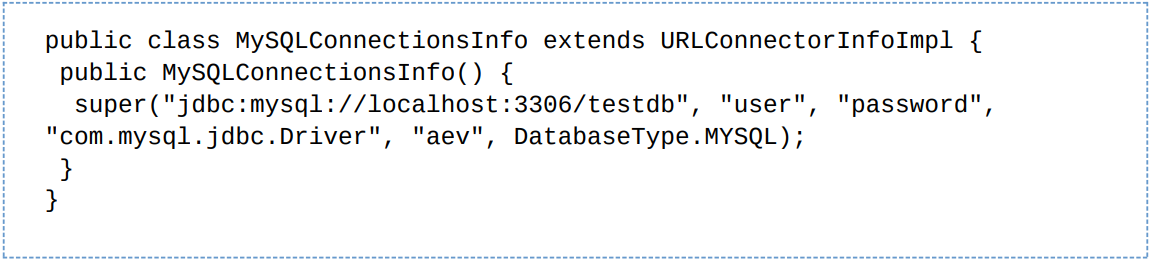
\includegraphics[width=0.8\textwidth]{images/gb/conInfo}
	\caption{ConnectionInfo konfigurieren}
	\label{img:gb/conInfo}
\end{figure}

Im nachhinein kann das Connector Repository konfiguriert werden. Dies enthält alle Konnektoren, die in der Datenbank Migration beteiligt sind. \\
\begin{figure}[H]
	\centering
	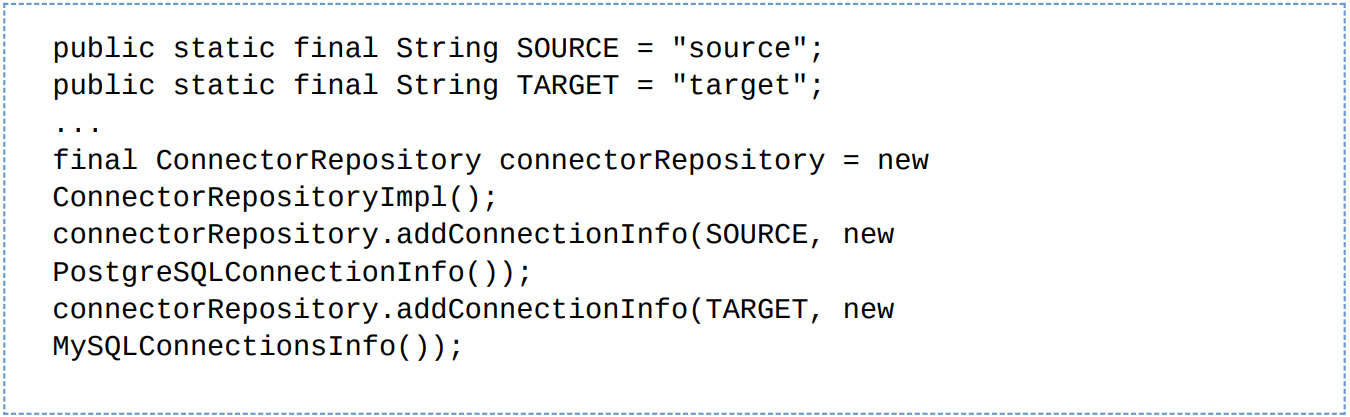
\includegraphics[width=0.8\textwidth]{images/gb/repo}
	\caption{Connector Repository konfigurieren}
	\label{img:gb/repo}
\end{figure}

\subsubsection*{Schritt 2: Hinweise hinzufügen}
Meistens werden Konfigurationshinweise (hints) benötigt, um die Migration zu individualisieren. In der Dokumentation von GuttenBase\footnote{Getting Started with GuttenBase (2018, 04.01) \\ \url{https://github.com/akquinet/GuttenBase/blob/master/Getting\%20Started\%20with\%20GuttenBase.pdf}} befindet sich eine Liste aller unterstützen Konfigurationshinweise. \\
Als Beispiel wird der Konfigurationshinweis ColumnMapperHint in der Abbildung dargestellt.
\begin{figure}[H]
	\centering
	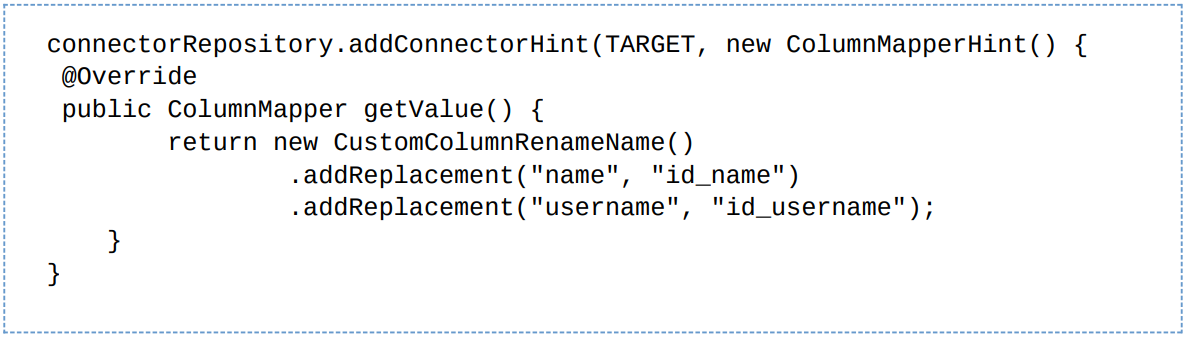
\includegraphics[width=0.8\textwidth]{images/gb/rename}
	\caption{ColumnMapperHint hinzufügen}
	\label{img:gb/rename}
\end{figure}


\subsubsection*{Schritt 3: Datenbank Migration durchführen}
Anschließend kann die Migration mit den eventuell hinzugefügten Hinweisen durchgeführt werden. Dies passiert wie folgt:
\begin{itemize}
	\item Das Datenbank Schema wird von der Quell-Datenbank in die Ziel-Datenbank kopiert. Dabei werden möglichst viele Unterschiede in Datentypdarstellung standardmäßig berücksichtigt.
	\item Die Kompatibilität von den Schemata wird geprüft. Hierbei wird nach gleichen Tabellen bzw Spalten gesucht.
	\item Falls es keine Fehler beim Prüfen gibt, werden die Daten dann kopiert.
\end{itemize}
\begin{figure}[H]
	\centering
	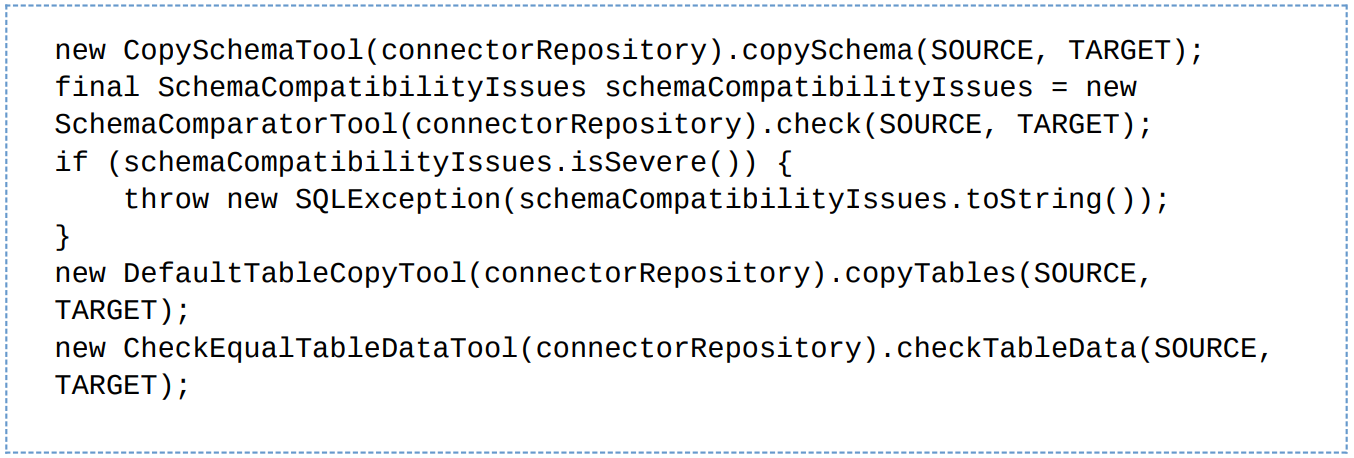
\includegraphics[width=0.8\textwidth]{images/gb/copy}
	\caption{Datenbank Migration durchführen}
	\label{img:gb/copy}
\end{figure}

%- Allgemeiner Satz
%- Was ist GuttenBase
%- Wann wurde sie eingeführt?
%- Von wem ist sie entwickelt?
%- Warum soll man GuttenBase benutzten
%- Wie kann man GuttenBase benutzen?
%- [Was kann man in GuttenBase optimieren?]


